
Este capítulo apresenta a abordagem metodológica adotada para o desenvolvimento da plataforma web proposta neste trabalho, detalhando a arquitetura do Ambiente de Desenvolvimento Integrado (IDE), as estratégias empregadas para a customização dinâmica de tokens e sintaxe, os mecanismos de integração com o núcleo do interpretador e os fluxos de execução, avaliação e \textit{feedback} ao usuário. A condução do trabalho seguiu rigorosamente as etapas previstas no cronograma do projeto, contemplando, nesta primeira fase do Trabalho de Conclusão de Curso, a revisão bibliográfica, a especificação do escopo dos comandos dinâmicos, a modelagem da arquitetura da plataforma, a implementação da customização interativa da linguagem, a execução das análises léxica e sintática a partir do código produzido na IDE, a apresentação dos resultados intermediários no terminal embutido e a finalização dos fluxos principais, com atenção à acessibilidade e à responsividade.

O desenvolvimento foi conduzido de forma incremental e iterativa, em conformidade com os princípios do desenvolvimento ágil discutidos por \citeonline{agile2012} e \citeonline{sabbagh2014}. Em razão da elevada quantidade de telas, componentes interativos e estados compartilhados característicos de uma IDE web, cada fluxo da plataforma, desde a autenticação do usuário até a submissão de exercícios, foi tratado como uma unidade autônoma de entrega, modelada, implementada e validada antes da agregação à etapa seguinte. Essa abordagem foi sustentada por testes automatizados unitários e de integração escritos com o \textit{framework} Vitest, conforme as práticas de Desenvolvimento Guiado por Testes consolidadas por \citeonline{aniche2012} e \citeonline{martin_coder}, permitindo a verificação contínua de regressões diante das frequentes mudanças impostas pela natureza altamente interativa da plataforma.

\section{Modelagem da Arquitetura da Plataforma}
\label{sec:arquitetura-plataforma}

A organização da plataforma foi concebida sob a ótica da Separação de Responsabilidades defendida por \citeonline{martin_clean}, dividindo o projeto em três camadas independentes e bem delimitadas: o pacote \texttt{compiler}, responsável pelo núcleo do interpretador; o pacote \texttt{ide}, responsável pela camada de apresentação e por toda a interação com o usuário; e o serviço de \textit{back-end}, responsável pela persistência das entidades de domínio do Ambiente Virtual de Aprendizagem. Os pacotes \texttt{compiler} e \texttt{ide} são versionados em um único repositório no formato \textit{monorepo}, viabilizando o consumo direto do compilador como dependência local da IDE, sem qualquer empacotamento intermediário e sem comunicação remota entre as duas camadas. Essa decisão arquitetural reduz drasticamente a latência da execução de programas no navegador e simplifica a propagação de mudanças no compilador para a interface.

O \textit{front-end} foi implementado com o \textit{framework} Next.js, em sua arquitetura de \textit{Pages Router}, sobre a biblioteca React 19, utilizando TypeScript em todo o código-fonte para garantir a verificação estática de tipos discutida por \citeonline{martin_clean_code}. A estilização foi conduzida com Tailwind CSS em sua quarta versão, complementada por componentes acessíveis das bibliotecas \textit{shadcn/ui} e \textit{Radix UI}, escolhidos por implementarem as recomendações da \textit{Web Accessibility Initiative} (WAI-ARIA) por padrão. O gerenciamento de estado assíncrono foi delegado à biblioteca \textit{TanStack React Query}, responsável pela orquestração de cache, sincronização e revalidação dos dados consumidos das rotas HTTP, enquanto a validação de formulários foi modelada com a biblioteca \textit{Zod}, integrada ao \textit{React Hook Form}.

A camada de \textit{back-end} foi implementada em Python sobre o \textit{framework} FastAPI, escolhido pelas características de alto desempenho, validação automática via \textit{Pydantic} e geração automatizada de documentação OpenAPI discutidas por \citeonline{fastapi2026}. A persistência foi sustentada pelo ORM SQLAlchemy assíncrono, com versionamento de \textit{schema} via Alembic, isolando o modelo de dados das regras de negócio em conformidade com os princípios de Arquitetura Limpa apresentados por \citeonline{martin_clean}. Essa separação garante que o banco de dados seja tratado estritamente como um detalhe de infraestrutura, permitindo que o núcleo de compilação e a interface web permaneçam agnósticos em relação à camada de armazenamento.

O fluxo geral de comunicação entre as camadas, ilustrado pela Figura \ref{fig:arquitetura-plataforma}, foi estruturado de modo que a execução do código submetido pelo usuário ocorra integralmente nos limites do servidor Next.js. A IDE invoca rotas HTTP locais sob o caminho \texttt{/api}, que importam diretamente as classes \texttt{Lexer}, \texttt{TokenIterator} e \texttt{Interpreter} do pacote \texttt{compiler}. As requisições destinadas à persistência são, por sua vez, delegadas ao serviço FastAPI por meio do cliente HTTP \textit{axios}. Essa segregação confere à plataforma a flexibilidade de executar programas mesmo na ausência de conexão com o serviço de persistência, mantendo plenamente funcionais os recursos de edição, análise léxica, geração de código intermediário e interpretação.

\begin{figure}[H]
    \centering
    \caption{Arquitetura geral da plataforma e fluxos de comunicação entre as camadas.}
    \label{fig:arquitetura-plataforma}
    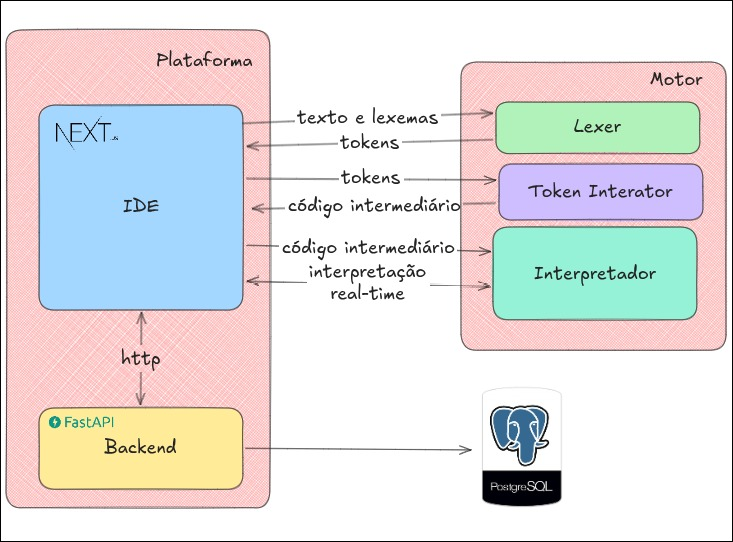
\includegraphics[width=0.95\textwidth]{Figuras/arquitetura-plataforma.jpeg}
    \legend{Fonte: elaborado pelo autor.}
\end{figure}

A organização interna do código da IDE seguiu a topologia clássica de aplicações Next.js, com diretórios dedicados para páginas (\texttt{pages}), componentes reutilizáveis (\texttt{components}), \textit{contexts} de estado global (\texttt{contexts}), \textit{hooks} personalizados (\texttt{hooks}), entidades de domínio (\texttt{entities}), bibliotecas de apoio (\texttt{lib}) e composições de tela (\texttt{views}). Essa segmentação materializa o princípio da coesão funcional discutido por \citeonline{silveira2012}, isolando responsabilidades específicas em módulos compactos e favorecendo tanto a legibilidade quanto a testabilidade do sistema.

\section{Interpretador}
\label{sec:interpretador-nucleo}

O interpretador constitui o núcleo de tradução comum a este projeto e foi desenvolvido de forma colaborativa pelos dois autores, Victor de Souza Vilela da Silva e Igor Lamoia Queiroz, conforme a divisão de responsabilidades registrada no Apêndice~\ref{ap:plano}. Implementado em TypeScript e consumido pela IDE como dependência local, conforme descrito na Seção~\ref{sec:arquitetura-plataforma}, o núcleo encadeia as fases de análise léxica, análise sintática, geração de código intermediário em três endereços e execução pelo interpretador, recebendo dinamicamente a configuração da linguagem definida pelo usuário (palavras-chave, operadores em forma de palavra, literais booleanos, delimitadores de bloco e terminador de instrução).

Por se tratar da base técnica compartilhada entre os dois volumes, o detalhamento interno de cada fase do núcleo, incluindo as estratégias de varredura léxica, a análise sintática por descida recursiva, a geração de código de três endereços e o funcionamento do interpretador, é objeto do trabalho complementar de autoria de Victor de Souza Vilela da Silva. Este volume concentra-se na forma como a IDE aciona e integra esse núcleo, detalhada nas seções seguintes.

\section{Customização Dinâmica de Tokens e Sintaxe}
\label{sec:customizacao-dinamica}

A funcionalidade central da plataforma, que consiste na possibilidade de o usuário personalizar dinamicamente a sintaxe e o vocabulário da linguagem, foi materializada em um conjunto coordenado de componentes, \textit{contexts} e utilitários. O elemento central dessa funcionalidade é o \texttt{KeywordContext}, um \textit{context} do React que mantém, em memória e na camada de armazenamento local do navegador, o estado completo da customização ativa, incluindo o mapeamento de palavras-chave personalizadas, os operadores em forma de palavra, os literais booleanos, os delimitadores de bloco e o terminador de instrução.

O contrato técnico que sustenta a customização é definido pelo módulo \texttt{config.ts} do pacote \texttt{compiler}, que declara, por meio de tipos TypeScript, todos os elementos da linguagem passíveis de personalização. O Trecho de Código~\ref{lst:lexer-config} apresenta esses tipos, que funcionam como a interface formal entre a camada de interface, responsável pela coleta das preferências do usuário, e o núcleo do tradutor, responsável pela construção da gramática efetiva no momento da varredura léxica.

\begin{lstlisting}[language=typescript, caption={Tipos que descrevem a configuração customizável do lexer.}, label={lst:lexer-config}, captionpos=b]
export type KeywordMap = Record<string, number>;

export type OperatorWordMap = {
  logical_or?: string;     logical_and?: string;
  logical_not?: string;    less?: string;
  less_equal?: string;     greater?: string;
  greater_equal?: string;  equal_equal?: string;
  not_equal?: string;
};

export type BooleanLiteralMap = {
  true?: string;
  false?: string;
};

export type LexerBlockDelimiters = {
  open: string;
  close: string;
};

export type LexerConfig = {
  customKeywords?: KeywordMap;
  operatorWordMap?: OperatorWordMap;
  booleanLiteralMap?: BooleanLiteralMap;
  statementTerminatorLexeme?: string;
  blockDelimiters?: LexerBlockDelimiters;
  locale?: string;
  indentationBlock?: boolean;
  tabWidth?: number;
};
\end{lstlisting}

A definição de quais elementos da linguagem seriam exibidos como configuráveis foi guiada pelos achados empíricos de \citeonline{stefik2013}, segundo os quais a sintaxe tradicional derivada da família C atua como uma barreira significativa para estudantes iniciantes. Foram disponibilizadas para customização as palavras-chave de declarações de tipo (\texttt{int}, \texttt{float}, \texttt{bool}, \texttt{string}), de controle de fluxo (\texttt{if}, \texttt{else}, \texttt{for}, \texttt{while}, \texttt{break}, \texttt{continue}, \texttt{return}, \texttt{switch}, \texttt{case}), as operações de entrada e saída (\texttt{print}, \texttt{scan}), os operadores lógicos (\texttt{\&\&}, \texttt{||}, \texttt{!}) e relacionais (\texttt{==}, \texttt{!=}, \texttt{>}, \texttt{>=}, \texttt{<}, \texttt{<=}), os literais booleanos (\texttt{true}, \texttt{false}), os delimitadores de bloco (chaves ou indentação) e o terminador de instrução. Essas opções abrangem precisamente os elementos que oneram a carga cognitiva inicial discutidos por \citeonline{stefik2013}, mantendo intactos os aspectos estruturais responsáveis pela consistência das demais fases do compilador.

A consolidação do estado da customização no \texttt{KeywordContext} é exposta às demais camadas da aplicação por meio do utilitário \texttt{buildLexerConfig}, apresentado no Trecho de Código~\ref{lst:build-lexer-config}. Esse utilitário traduz o estado em memória, contendo os mapeamentos de palavras-chave, os operadores, os literais booleanos, os delimitadores de bloco e o terminador de instrução, em um descritor compatível com o tipo \texttt{LexerConfig} do pacote \texttt{compiler}, atuando como a fronteira efetiva entre o estado da interface e a invocação do tradutor.

\begin{lstlisting}[language=typescript, caption={Utilitário \texttt{buildLexerConfig} do \texttt{KeywordContext}, que materializa a configuração corrente em um descritor consumível pelo lexer.}, label={lst:build-lexer-config}, captionpos=b]
const buildKeywordMap = useCallback((): Record<string, number> => {
  const map: Record<string, number> = {};
  for (const m of customization.mappings) {
    map[m.custom] = m.tokenId;
  }
  return map;
}, [customization.mappings]);

const buildLexerConfig = useCallback((): IDECompilerConfigPayload => {
  return buildLexerConfigFromCustomization(customization);
}, [customization]);
\end{lstlisting}

A interface de customização foi implementada como um assistente progressivo no formato \textit{wizard}, materializado no componente \texttt{keyword-customizer}, que conduz o usuário por etapas independentes, cada uma responsável por um aspecto específico da personalização. O fluxo é controlado pelo \texttt{wizard-model}, que mantém o estado de navegação e valida cada passo antes de permitir o avanço. A declaração formal das etapas do assistente é apresentada no Trecho de Código~\ref{lst:wizard-steps}, no qual cada elemento do arranjo \texttt{WIZARD\_STEPS} associa um identificador, um título exibido na barra de progresso, uma descrição textual e um ícone semântico, oferecendo ao usuário um mapa visual contínuo do fluxo de personalização.

\begin{lstlisting}[language=typescript, caption={Declaração do arranjo \texttt{WIZARD\_STEPS}, que organiza as etapas do assistente de personalização.}, label={lst:wizard-steps}, captionpos=b]
export const WIZARD_STEPS = [
  { id: "identity",  title: "Identidade",
    description: "Escolha o ponto de partida da linguagem.",
    icon: "fingerprint" },
  { id: "IO",        title: "Entrada/Saida",
    description: "Defina saida, leitura e a linguagem das variaveis.",
    icon: "cable" },
  { id: "types",     title: "Tipagem",
    description: "Defina leitura, escrita e o vocabulario usado para declarar variaveis.",
    icon: "book-open-text" },
  { id: "structure", title: "Estrutura",
    description: "Configure blocos, delimitadores e o fim das instrucoes.",
    icon: "blocks" },
  { id: "rules",     title: "Operadores",
    description: "Ajuste os operadores, literais booleanos e regras de decisao.",
    icon: "sigma" },
  { id: "flow",      title: "Fluxo",
    description: "Customize o vocabulario de controle.",
    icon: "route" },
  { id: "review",    title: "Revisao",
    description: "Confira o resumo final antes de salvar.",
    icon: "clipboard-check" },
] as const;
\end{lstlisting}

A cada alteração proposta pelo usuário, o componente \texttt{preview-builder} produz, em tempo real, um trecho de código exemplificativo que reflete a customização corrente, oferecendo uma visualização imediata do impacto das mudanças sobre a aparência dos programas. O Trecho de Código~\ref{lst:preview-builder} ilustra a função \texttt{buildDelimiterSnippet}, responsável por interpolar, em um molde fixo, as palavras-chave e os delimitadores efetivamente escolhidos pelo usuário, produzindo um pequeno programa exemplificativo coerente com a configuração corrente.

\begin{lstlisting}[language=typescript, caption={Função \texttt{buildDelimiterSnippet}, que gera o \textit{preview} dinâmico exibido durante a personalização.}, label={lst:preview-builder}, captionpos=b]
export function buildDelimiterSnippet(
  draft: StoredKeywordCustomization,
): string {
  const print = getKeyword(draft, "print");
  const scan = getKeyword(draft, "scan");
  const lineEnding = buildLineEnding(draft);
  const funcao = getKeyword(draft, "funcao");
  const baseCodeSnippet = `${funcao} main()`;

  const open = draft.blockDelimiters.open.trim() || "{";
  const close = draft.blockDelimiters.close.trim() || "}";

  return `${baseCodeSnippet}${open}\n\t${print}("Ola Mundo!")${lineEnding}
  ${scan}(nome)${lineEnding}\n\t${print}("Me chamo:", nome)\n${close}`;
}
\end{lstlisting} Essa estratégia de \textit{feedback} contínuo segue as recomendações de \citeonline{nystrom2021} para ambientes interativos de aprendizagem, reduzindo a distância cognitiva entre a configuração e o resultado observável.

A validação das customizações é centralizada em um conjunto de funções utilitárias dedicadas, hospedadas no diretório \texttt{contexts/keyword/keyword-validator.ts}. A função \texttt{validateCustomKeyword} garante que palavras-chave personalizadas atendam às restrições léxicas elementares e não colidam entre si; \texttt{validateBlockDelimiters} verifica a consistência dos delimitadores de bloco. Toda a verificação ocorre de forma preventiva, no momento da alteração pelo usuário, impedindo que configurações inválidas sejam persistidas ou propagadas ao analisador léxico, em conformidade com os princípios de detecção precoce de erros discutidos por \citeonline{cooper2012}.

O Trecho de Código~\ref{lst:validate-delimiters} ilustra a estratégia de verificação aplicada aos delimitadores de bloco. A função encadeia as restrições elementares (ambos os delimitadores preenchidos, conformidade com o formato de identificadores, distinção entre o delimitador de abertura e o de fechamento e ausência de colisão com palavras reservadas), devolvendo, em caso de violação, a mensagem internacionalizada correspondente. Quando todas as restrições são atendidas, a função retorna \texttt{null}, sinalizando à interface que a configuração pode ser persistida.

\begin{lstlisting}[language=typescript, caption={Função \texttt{validateBlockDelimiters}, responsável pela verificação preventiva dos delimitadores de bloco.}, label={lst:validate-delimiters}, captionpos=b]
export function validateBlockDelimiters(
  value: BlockDelimiters,
): string | null {
  const open = value.open.trim();
  const close = value.close.trim();

  if (!open && !close) return null;
  if (!open || !close) {
    return ui.validation_fill_delimiters;
  }

  if (!WORD_REGEX.test(open) || !WORD_REGEX.test(close)) {
    return ui.validation_invalid_delimiter_format;
  }

  if (open === close) {
    return ui.validation_delimiters_must_differ;
  }

  if (
    ORIGINAL_KEYWORDS.includes(open) ||
    ORIGINAL_KEYWORDS.includes(close)
  ) {
    return ui.validation_delimiters_reserved;
  }

  return null;
}
\end{lstlisting}

A persistência da customização foi modelada em duas camadas complementares. As configurações ativas no editor são salvas localmente, no \textit{localStorage} do navegador, por meio do utilitário \texttt{keyword-language-storage}, garantindo que o estado da personalização sobreviva ao recarregamento da página e à navegação entre rotas da aplicação. Linguagens nomeadas e exportadas pelo usuário, por sua vez, são persistidas no \textit{back-end} via API, viabilizando o compartilhamento entre dispositivos e a vinculação de linguagens específicas a exercícios oferecidos pelo professor. O utilitário \texttt{language-creator-navigation} orquestra as transições entre as etapas de criação, gravação e ativação de linguagens, mantendo coesão entre o estado em memória, o estado no \textit{localStorage} e o estado remoto.

Por fim, o impacto visual imediato da customização sobre o editor Monaco é mediado pela função \texttt{updateJavaMMKeywords}. Essa função reconstrói dinamicamente a gramática léxica registrada no editor cada vez que o \texttt{KeywordContext} sinaliza uma alteração na customização, refletindo de imediato o realce de sintaxe, a sugestão automática de palavras-chave e a documentação contextual exibida pelo Monaco. O Trecho de Código~\ref{lst:update-monaco} apresenta sua assinatura, evidenciando o desacoplamento entre o módulo de personalização e o módulo de edição: a função recebe a instância do Monaco, o conjunto atualizado de mapeamentos e as opções de linguagem, delegando à função interna \texttt{registerJavaMMLanguage} o registro completo do dialeto sob o identificador \texttt{java--}. Essa abordagem evita a necessidade de reinicializar o editor a cada mudança e oferece ao usuário uma sensação de continuidade absoluta no ato de personalização.

\begin{lstlisting}[language=typescript, caption={Função \texttt{updateJavaMMKeywords}, ponto de integração entre o estado da customização e o Monaco Editor.}, label={lst:update-monaco}, captionpos=b]
export const JAVAMM_LANGUAGE_ID = "java--";

export type JavaMMKeywordMapping = {
  original: string;
  custom: string;
  tokenId: number;
};

export function updateJavaMMKeywords(
  monaco: typeof monacoEditor,
  keywordMappings: JavaMMKeywordMapping[],
  options: JavaMMLanguageOptions = {},
) {
  registerJavaMMLanguage(monaco, keywordMappings, options);
}
\end{lstlisting}

\section{Edição de Código e Sistema de Arquivos Virtual}
\label{sec:edicao-codigo}

A experiência de edição foi construída em torno do \textit{Microsoft Monaco Editor}, o mesmo motor de edição utilizado pelo Visual Studio Code, integrado à aplicação por meio do pacote \texttt{@monaco-editor/loader}. A linguagem personalizada do projeto foi registrada sob o identificador \texttt{java--}, e dois temas próprios, \texttt{editor-glass-dark} e \texttt{editor-glass-light}, foram modelados a partir do módulo \texttt{EditorThemes.ts} para harmonizar visualmente o editor com o restante da identidade da plataforma, em ambas as variações de tema claro e escuro.

O gerenciamento do editor foi encapsulado no \texttt{EditorContext}, que abriga a referência da instância Monaco, o código-fonte corrente, o nome do arquivo ativo, os marcadores de linha utilizados para destacar erros e o conjunto de configurações de exibição. A interação entre o usuário e o editor foi enriquecida pelo \textit{hook} \texttt{useDebugger}, responsável por sinalizar visualmente, durante a execução passo a passo, qual instrução do código intermediário está sendo processada pelo interpretador, em consonância com o requisito pedagógico de tornar visível o processo de tradução.

A persistência local dos arquivos do usuário foi modelada pelo \textit{hook} \texttt{useFileSystem}, que implementa um sistema de arquivos virtual sustentado pelo \textit{localStorage} do navegador. Essa abordagem permite que múltiplos arquivos sejam criados, renomeados, removidos e alternados sem qualquer dependência de servidor remoto, mantendo a plataforma plenamente funcional inclusive em cenários de uso \textit{offline}. O \textit{hook} \texttt{useEditorWithFileSystem} combina o estado do editor com o sistema de arquivos virtual, garantindo a sincronização bidirecional entre o conteúdo exibido no Monaco e o conteúdo persistido localmente. Complementarmente, os \textit{hooks} \texttt{useExplorer} e \texttt{useSearch} oferecem, no painel lateral, navegação por estrutura de arquivos e busca textual sobre todos os arquivos do projeto, replicando as funcionalidades essenciais de uma IDE profissional.

\section{Execução das Análises Léxica e Sintática a partir da IDE}
\label{sec:execucao-analises}

A invocação das análises do compilador a partir da IDE foi modelada por meio de \textit{hooks} dedicados que encapsulam toda a interação entre a camada de interface e o núcleo de tradução. Diferentemente da estratégia adotada por ferramentas como a plataforma Laila, discutida no referencial teórico, na qual o código submetido pelo usuário é encaminhado a um serviço remoto para processamento, neste trabalho a execução das análises foi modelada inteiramente no navegador, sem intermediação de rotas HTTP. Essa decisão arquitetural foi viabilizada pela organização \textit{monorepo} descrita na Seção~\ref{sec:arquitetura-plataforma}, que permite à IDE consumir o pacote \texttt{compiler} como dependência local e instanciar suas classes diretamente no contexto de execução do cliente.

O \textit{hook} \texttt{useLexerAnalyse} concentra a orquestração da fase léxica. A cada solicitação do usuário, o \textit{hook} recupera o código-fonte corrente, consulta o \texttt{KeywordContext} para obter a configuração ativa da linguagem dinâmica, normaliza o mapeamento efetivo de palavras-chave por meio do utilitário \texttt{buildEffectiveKeywordMap} e instancia uma nova classe \texttt{Lexer} do pacote \texttt{compiler}, passando como parâmetros o mapa de palavras-chave personalizadas, os operadores em forma de palavra, os literais booleanos, o terminador de instrução, os delimitadores de bloco e o \textit{locale} ativo. A varredura é então executada pelo método \texttt{scanTokens}, e a coleção de \textit{tokens} resultante, juntamente com eventuais avisos e mensagens informativas coletadas pelo sistema de \textit{issues}, é devolvida diretamente ao componente que originou a invocação, sem qualquer ida ao servidor.

O Trecho de Código~\ref{lst:run-lexer} evidencia essa instanciação direta. Observa-se a importação do símbolo \texttt{Lexer} a partir do pacote local \texttt{@ts-compilator-for-java/compiler}, viabilizada pela organização em \textit{monorepo}, e a construção do analisador com a configuração derivada do \texttt{KeywordContext}, sem qualquer chamada HTTP intermediária.

\begin{lstlisting}[language=typescript, caption={Função \texttt{runLexerAnalyse}, que instancia o lexer diretamente no cliente.}, label={lst:run-lexer}, captionpos=b]
import { Lexer } from "@ts-compilator-for-java/compiler/src/lexer";

async function runLexerAnalyse(
  input: RunLexerAnalyseInput,
): Promise<TLexerAnalyseData> {
  try {
    const effectiveKeywordMap = buildEffectiveKeywordMap(input.keywordMap);
    const lexer = new Lexer(input.sourceCode, {
      customKeywords: effectiveKeywordMap,
      operatorWordMap: input.operatorWordMap,
      booleanLiteralMap: input.booleanLiteralMap,
      statementTerminatorLexeme: input.statementTerminatorLexeme,
      blockDelimiters: input.blockDelimiters,
      locale: input.locale,
      indentationBlock: input.indentationBlock,
    });
    const tokens = lexer.scanTokens();
    return {
      message: "Lexical Analysis completed",
      tokens,
      warnings: lexer.warnings,
      infos: lexer.infos,
      error: null,
    };
  } catch (error) {
    if (error instanceof IssueError) throw error;
    throw new Error((error as Error).message || "Codigo nao suportado");
  }
}
\end{lstlisting}

Os \textit{tokens} obtidos por essa execução local são renderizados na IDE como cartões interativos pelo componente \texttt{token-card}, oferecendo ao usuário uma visualização direta do resultado da fase léxica, incluindo o lexema original, sua categoria e sua posição no código-fonte. Essa exposição direta atende ao propósito pedagógico de tornar visíveis as etapas internas do processo de tradução, característica diferencial da plataforma em relação às ferramentas analisadas no referencial teórico. Eventuais erros lançados pelo lexer, encapsulados pela classe \texttt{IssueError}, são interceptados pelo \textit{hook} e materializados tanto no terminal quanto no editor, por meio dos utilitários \texttt{showLineIssues} e do mecanismo de marcadores discutido na Seção~\ref{sec:terminal-feedback}.

O \textit{hook} \texttt{useIntermediatorCode} segue uma abordagem análoga. Após reaproveitar a tabela de \textit{tokens} produzida pela fase léxica, o \textit{hook} instancia um \texttt{TokenIterator} e aciona o analisador sintático diretamente no cliente, integrado a um \texttt{Emitter} responsável pela geração das instruções de código intermediário em três endereços. A lista de instruções resultante é igualmente exibida na IDE em um painel dedicado, permitindo ao estudante inspecionar a tradução do código-fonte para uma forma de representação intermediária. Essa execução também ocorre integralmente no navegador, sem qualquer requisição HTTP intermediária.

A escolha por executar as análises léxica e sintática diretamente no cliente, em vez de delegá-las ao servidor por meio de rotas internas do Next.js, atende a três objetivos correlacionados. Primeiro, minimiza a latência percebida pelo usuário, ao eliminar o ciclo de requisição e resposta exigido por uma arquitetura cliente-servidor convencional. Segundo, permite que a plataforma permaneça plenamente funcional mesmo na ausência de conectividade com o servidor de persistência, sustentando os recursos essenciais de edição, análise e interpretação. Terceiro, simplifica a manutenção do código, uma vez que a lógica do compilador é consumida como dependência direta, sem necessidade de empacotamento, serialização ou conversão de tipos entre cliente e servidor. As rotas HTTP do servidor Next.js, situadas sob o caminho \texttt{/api}, são reservadas exclusivamente ao subsistema de validação automatizada de submissões e à intermediação das chamadas ao \textit{back-end} FastAPI, conforme detalhado na Seção~\ref{sec:sistema-correcao}.

Por fim, o \textit{hook} \texttt{use-api-queries} consolida, por meio do \textit{TanStack React Query}, todas as consultas relacionadas a turmas, exercícios, listas de exercícios e submissões, oferecendo cache automático, revalidação em segundo plano e tratamento padronizado de erros para toda a aplicação. Essas consultas, distintamente das análises locais discutidas anteriormente, são as únicas que envolvem comunicação remota efetiva com o serviço de persistência, mantendo claras as fronteiras entre a execução local do compilador e o consumo de recursos do Ambiente Virtual de Aprendizagem.

\section{Execução do Código Intermediário e \textit{Feedback} no Terminal}
\label{sec:terminal-feedback}

O componente \texttt{terminal}, hospedado em \texttt{components/terminal}, foi modelado como o canal primário de \textit{feedback} interativo entre o programa em execução e o usuário. Sua arquitetura interna é composta por três peças: o componente \texttt{body}, que renderiza o histórico de saídas e o prompt de entrada; o componente \texttt{header}, que apresenta os controles de execução e o estado corrente; e o \textit{hook} \texttt{useKeyboardShortcuts}, que mapeia atalhos teclados às operações de limpeza, foco e interrupção da execução. O terminal é controlado pelo \texttt{TerminalContext}, responsável por gerenciar seu estado de abertura, fechamento e visibilidade na composição da tela.

A execução dos programas foi modelada de modo que as operações \texttt{print} e \texttt{scan} produzidas pelo interpretador sejam diretamente conectadas ao terminal embutido. O \texttt{Interpreter}, instanciado no servidor Next.js, recebe funções de retorno (\texttt{stdout} e \texttt{stdin}) cujo comportamento varia conforme o modo de execução: em modo interativo, as funções são associadas ao terminal da IDE; em modo de validação automatizada de exercícios, são conectadas a \textit{buffers} controlados que capturam a saída para comparação com o resultado esperado. Esse desacoplamento entre o motor de execução e a camada de apresentação atende aos princípios de baixo acoplamento discutidos por \citeonline{martin_clean} e foi inspirado nas abstrações de fluxos de entrada e saída descritas por \citeonline{cooper2012}.

O sistema de \textit{feedback} de erros foi modelado em duas categorias complementares. Os erros estáticos detectados durante a compilação, como falhas léxicas, sintáticas e semânticas, são reportados pelo módulo \texttt{issue} do pacote \texttt{compiler}, que classifica cada ocorrência como \texttt{IssueError} (impede a tradução), \texttt{IssueWarning} (alerta não fatal) ou \texttt{IssueInfo} (informação contextual). Essas mensagens são interceptadas pela IDE e materializadas tanto no terminal, em formato textual, quanto no editor, por meio de marcadores de linha sublinhados, em conformidade com as práticas de relato de erros discutidas por \citeonline{aho1995}. Os erros dinâmicos, detectados pelo interpretador em tempo de execução (como divisões por zero, conversões impossíveis durante a leitura de entrada ou acessos a posições inválidas de \textit{arrays}), são encapsulados pela classe \texttt{RuntimeError} e gerenciados pelo \texttt{RuntimeErrorContext}, que coordena a exibição contextualizada no terminal e o destaque visual no editor.

Para garantir que mensagens de erro sejam pedagogicamente úteis, mesmo quando a linguagem corrente está fortemente personalizada, todas as mensagens passam pelo módulo de internacionalização \texttt{i18n} do pacote \texttt{compiler}, que oferece traduções para os idiomas \textit{pt-BR}, \textit{pt-PT}, \textit{es} e \textit{en}. Adicionalmente, as mensagens são adaptadas ao vocabulário corrente da customização: termos como ``palavra reservada esperada'' são substituídos pela palavra-chave efetivamente esperada na configuração ativa, evitando a exposição ao usuário de termos canônicos que tenham sido propositalmente ocultados pela personalização.

\section{Sistema de Correção e Avaliação Automatizada}
\label{sec:sistema-correcao}

A plataforma incorpora um subsistema de avaliação automatizada inspirado nos juízes \textit{online} discutidos por \citeonline{ferreira2025} e \citeonline{garcia2024}, materializado pela rota \texttt{/api/submissions/validate}. A modelagem do fluxo de submissão de exercícios partiu da estrutura conceitual desses juízes, mas foi adaptada ao contexto da linguagem dinâmica: enquanto os juízes tradicionais exigem que o aluno se adapte à sintaxe rígida de uma linguagem comercial, a plataforma proposta permite que cada exercício carregue sua própria configuração da linguagem, podendo, inclusive, restringir o aluno a um vocabulário específico definido pelo professor.


O modelo de dados que sustenta o Ambiente Virtual de Aprendizagem foi estruturado em torno das entidades \texttt{User}, \texttt{Class}, \texttt{Exercise}, \texttt{ExerciseList}, \texttt{Submission} e \texttt{LanguageImage}. Essa modelagem permite que professores criem turmas, vinculem exercícios estruturados em listas, definam casos de teste com entradas e saídas esperadas, e associem a cada exercício uma ``imagem de linguagem'', isto é, uma configuração da linguagem dinâmica que será imposta ao aluno no momento da resolução. As consultas e mutações sobre essas entidades são tratadas pelo \textit{back-end} FastAPI, com persistência em SQLAlchemy assíncrono, e gerenciadas no \textit{front-end} pelo \textit{TanStack React Query}, que cuida do cache e da revalidação automática.

\section{Acessibilidade, Responsividade e Finalização de Fluxos}
\label{sec:acessibilidade-responsividade}

A finalização dos fluxos da plataforma foi conduzida com especial atenção aos requisitos de acessibilidade e responsividade. A escolha das bibliotecas \textit{shadcn/ui} e \textit{Radix UI} como base dos componentes primitivos, incluindo diálogos, menus, \textit{tooltips}, alertas, abas e \textit{popovers}, garante, por padrão, o cumprimento das diretrizes WAI-ARIA, com suporte nativo à navegação por teclado, à leitura por tecnologias assistivas e ao gerenciamento correto de foco. Essa abordagem alinha-se aos princípios de design inclusivo discutidos por \citeonline{stefik2013} e \citeonline{ladner2019} na concepção da linguagem Quorum, segundo os quais a acessibilidade não pode ser uma camada adicional, mas deve estar incorporada à fundação dos componentes utilizados.

A responsividade da plataforma foi modelada pelo \textit{hook} \texttt{useBreakpoint}, que monitora as dimensões da janela e expõe, de forma reativa, qual \textit{breakpoint} Tailwind está ativo. As composições de tela, hospedadas no diretório \texttt{views}, foram concebidas para reorganizar dinamicamente seus painéis conforme a faixa de resolução: em telas amplas, o editor, o painel lateral e o terminal são apresentados simultaneamente; em telas estreitas, esses componentes assumem disposições alternativas, com a possibilidade de alternância controlada pelo usuário. Essa adaptação foi sustentada pelas utilidades de responsividade do Tailwind CSS v4 e pela função utilitária \texttt{cn}, que compõe classes condicionais com a biblioteca \textit{tailwind-merge}.

O tratamento de temas claro e escuro foi delegado à biblioteca \textit{next-themes}, integrada ao \texttt{ThemeContext}, que mantém o tema corrente sincronizado entre o sistema operacional do usuário, a preferência salva e os múltiplos componentes da aplicação. Os temas do editor Monaco são alternados de forma coordenada, garantindo consistência visual entre o ambiente de edição e o restante da interface. As notificações ao usuário, por sua vez, são gerenciadas pelo \texttt{ToastContext}, oferecendo uma fila padronizada de mensagens com diferentes níveis de severidade.

A internacionalização da plataforma foi implementada por meio do mecanismo nativo do Next.js, com suporte aos locais \textit{pt-BR} (padrão), \textit{pt-PT}, \textit{es} e \textit{en}, organizados em arquivos JSON sob o diretório \texttt{i18n/locales}. Todas as cadeias visíveis ao usuário foram externalizadas para esses arquivos, permitindo que a plataforma seja oferecida em diferentes idiomas e que o conteúdo pedagógico se ajuste ao público-alvo. Essa decisão atende à premissa central do projeto, segundo a qual barreiras linguísticas devem ser sistematicamente reduzidas no contexto da aprendizagem introdutória de programação.

A autenticação de usuários foi modelada por um fluxo simplificado, sustentado pelo \texttt{AuthContext} no \textit{front-end} e pelas rotas \texttt{/api/auth/login}, \texttt{/api/auth/register} e \texttt{/api/auth/me}. As credenciais são propagadas entre as camadas por meio de \textit{cookies} HTTP gerenciados pelo utilitário \texttt{auth-cookies}, e a navegação protegida é controlada pelos \textit{layouts} compartilhados, que verificam a presença de uma sessão válida antes de renderizar páginas restritas. Essa estratégia atende aos requisitos mínimos de segregação entre os papéis de aluno, professor e administrador, e mantém a complexidade do modelo de autenticação compatível com o caráter educacional do projeto.

\section{Apresentação das Telas da Plataforma}
\label{sec:telas-plataforma}

Com o intuito de tornar tangíveis as decisões arquiteturais, os \textit{contexts} de estado, os \textit{hooks} e os componentes discutidos ao longo das seções anteriores, esta seção apresenta as principais telas efetivamente implementadas até o encerramento desta etapa do trabalho. A organização segue o fluxo natural de uso da plataforma: parte-se da identidade visual da página inicial, percorrem-se os painéis dos perfis de aluno e de professor e, por fim, ilustra-se o passo a passo de criação e personalização de uma linguagem dinâmica diretamente na IDE.

\noindent\textbf{Página Inicial e Identidade Visual}

A página inicial materializa a identidade visual da plataforma e funciona como porta de entrada para os fluxos de autenticação, navegação e divulgação dos recursos disponíveis. A composição segue o sistema de temas claro e escuro discutido na Seção~\ref{sec:acessibilidade-responsividade}, com troca controlada pelo \texttt{ThemeContext}, e foi modelada com componentes da biblioteca \textit{shadcn/ui} para garantir consistência tipográfica, contraste adequado e respeito às diretrizes de acessibilidade WAI-ARIA. As Figuras~\ref{fig:home-light} e \ref{fig:home-dark} apresentam, lado a lado, as duas variações de tema, evidenciando o cuidado com a paridade visual entre as versões clara e escura.

\begin{figure}[h]
    \centering
    \begin{subfigure}{0.9\textwidth}
        \centering
        
\includegraphics[width=\textwidth]{home_page_light.png}
        \caption{Tema claro.}
        \label{fig:home-light}
    \end{subfigure}

    \vspace{0.8em}

    \begin{subfigure}{0.9\textwidth}
        \centering
        
\includegraphics[width=\textwidth]{home_page_dark.png}
        \caption{Tema escuro.}
        \label{fig:home-dark}
    \end{subfigure}
    \caption{Página inicial da plataforma em suas duas variações de tema.}
    \label{fig:home-page}
    \legend{Fonte: elaborado pelo autor.}
\end{figure}

\FloatBarrier

\noindent\textbf{Painel do Aluno}

O painel do aluno consolida, em uma única tela, todas as turmas em que o estudante está matriculado, as listas de exercícios pendentes e o histórico recente de submissões. A tela foi modelada para reduzir o número de cliques necessários até o exercício seguinte, oferecendo cartões interativos que conduzem o aluno diretamente à composição da IDE com a linguagem dinâmica já configurada pelo professor. A Figura~\ref{fig:painel-aluno} ilustra a disposição geral desse painel.

\begin{figure}[H]
    \centering
    
\includegraphics[width=0.85\textwidth]{Aluno/painel_aluno.png}
    \caption{Painel principal do aluno, com acesso às turmas, listas e exercícios.}
    \label{fig:painel-aluno}
    \legend{Fonte: elaborado pelo autor.}
\end{figure}

Ao selecionar uma turma específica, o aluno é conduzido à tela de detalhamento, na qual visualiza informações da disciplina, listas publicadas pelo professor e seu progresso individual em cada exercício. A Figura~\ref{fig:aluno-turma} apresenta essa visão, enquanto a Figura~\ref{fig:aluno-listas} detalha a estrutura interna de uma lista de exercícios, na qual cada item exibe o respectivo estado (não iniciado, em andamento ou submetido) e a configuração da linguagem dinâmica vinculada ao enunciado.

\begin{figure}[h]
    \centering
    \begin{subfigure}{0.9\textwidth}
        \centering
        
\includegraphics[width=\textwidth]{Aluno/detail_turma.png}
        \caption{Detalhamento de uma turma do aluno.}
        \label{fig:aluno-turma}
    \end{subfigure}

\end{figure}

\begin{figure}[h]\ContinuedFloat

    \begin{subfigure}{0.9\textwidth}
        \centering
        
\includegraphics[width=\textwidth]{Aluno/Listas/Listas.png}
        \caption{Lista de exercícios sob a ótica do aluno.}
        \label{fig:aluno-listas}
    \end{subfigure}
    \caption{Composições da experiência do aluno: visão da turma e visão da lista de exercícios.}
    \label{fig:aluno-fluxo}
    \legend{Fonte: elaborado pelo autor.}
\end{figure}

\FloatBarrier

\noindent\textbf{Painel do Professor}

O painel do professor segue a mesma metáfora de organização do painel do aluno, mas amplia o conjunto de ações disponíveis, incorporando criação e gestão de turmas, listas de exercícios e enunciados. A Figura~\ref{fig:painel-professor} apresenta a visão consolidada do professor, com acesso direto às turmas sob sua responsabilidade. Ao selecionar uma turma, são exibidas as listas associadas, conforme a Figura~\ref{fig:professor-turma}, e o conjunto de listas pode ser inspecionado em maior detalhe pela visão dedicada da Figura~\ref{fig:professor-listas-turma}.

\begin{figure}[H]
    \centering
    
\includegraphics[width=0.85\textwidth]{Professor/painel_professor.png}
    \caption{Painel principal do professor.}
    \label{fig:painel-professor}
    \legend{Fonte: elaborado pelo autor.}
\end{figure}

\begin{figure}[h]
    \centering
    \begin{subfigure}{0.9\textwidth}
        \centering
        
\includegraphics[width=\textwidth]{Professor/detail_turma.png}
        \caption{Detalhamento de uma turma do professor.}
        \label{fig:professor-turma}
    \end{subfigure}

\end{figure}

\begin{figure}[h]\ContinuedFloat
\centering
    \begin{subfigure}{0.9\textwidth}
        \centering
        
\includegraphics[width=\textwidth]{Professor/listas_turma.png}
        \caption{Listas de exercícios vinculadas à turma.}
        \label{fig:professor-listas-turma}
    \end{subfigure}
    \caption{Composições da experiência do professor: visão da turma e visão das listas associadas.}
    \label{fig:professor-fluxo-turma}
    \legend{Fonte: elaborado pelo autor.}
\end{figure}

\FloatBarrier

\subsubsection*{Gerenciamento de Listas e Exercícios}

A criação e a manutenção de listas pelo professor ocorrem em telas dedicadas que isolam cada operação em um fluxo independente. A Figura~\ref{fig:professor-listas-fluxo} reúne, em uma única composição, as quatro etapas centrais desse processo: a visualização das listas existentes, a configuração dos parâmetros gerais da lista (título, descrição e prazo), a vinculação de exercícios à lista por meio do utilitário de busca e seleção, e a publicação da lista para a turma escolhida.

\begin{figure}[h]
    \centering

    \begin{subfigure}{0.9\textwidth}
        \centering
        
\includegraphics[width=\textwidth]{Professor/Listas/list.png}
        \caption{Listagem das listas existentes.}
        \label{fig:prof-lista-list}
    \end{subfigure}

    \vspace{0.8em}

    \begin{subfigure}{0.9\textwidth}
        \centering
        
\includegraphics[width=\textwidth]{Professor/Listas/config.png}
        \caption{Configuração dos parâmetros gerais.}
        \label{fig:prof-lista-config}
    \end{subfigure}

\end{figure}

\begin{figure}[p]\ContinuedFloat
    \centering

    \begin{subfigure}{0.9\textwidth}
        \centering
        
\includegraphics[width=\textwidth]{Professor/Listas/add_exec.png}
        \caption{Vinculação de exercícios à lista.}
        \label{fig:prof-lista-add}
    \end{subfigure}

    \vspace{0.8em}

    \begin{subfigure}{0.9\textwidth}
        \centering
        
\includegraphics[width=\textwidth]{Professor/Listas/publish.png}
        \caption{Publicação da lista para a turma.}
        \label{fig:prof-lista-publish}
    \end{subfigure}

    \caption{Fluxo de criação e gestão de listas de exercícios pelo professor.}
    \label{fig:professor-listas-fluxo}
    \legend{Fonte: elaborado pelo autor.}
\end{figure}

\FloatBarrier

A gestão dos enunciados individuais ocorre em um conjunto análogo de telas, ilustrado pela Figura~\ref{fig:professor-exercicios-fluxo}. A tela de listagem permite a busca, a filtragem e a ordenação dos enunciados; a tela de criação centraliza, em um único formulário, a descrição do problema, os casos de teste com entradas e saídas esperadas e a vinculação a uma imagem de linguagem que delimita o vocabulário disponível ao aluno; a tela de detalhamento mostra a composição final do exercício; e a tela de submissões consolida todas as resoluções enviadas pelos alunos, com os respectivos vereditos do subsistema de avaliação automatizada discutido na Seção~\ref{sec:sistema-correcao}.

\begin{figure}[h]
    \centering
    \begin{subfigure}{0.9\textwidth}
        \centering
        
\includegraphics[width=\textwidth]{Professor/Exercicios/list.png}
        \caption{Listagem dos enunciados existentes.}
        \label{fig:prof-exec-list}
    \end{subfigure}

    \vspace{0.8em}

    \begin{subfigure}{0.9\textwidth}
        \centering
        
\includegraphics[width=\textwidth]{Professor/Exercicios/create.png}
        \caption{Criação de um novo enunciado.}
        \label{fig:prof-exec-create}
    \end{subfigure}

\end{figure}

\begin{figure}[p]\ContinuedFloat
    \centering

    \begin{subfigure}{0.9\textwidth}
        \centering
        
\includegraphics[width=\textwidth]{Professor/Exercicios/detail.png}
        \caption{Detalhamento de um exercício.}
        \label{fig:prof-exec-detail}
    \end{subfigure}

    \vspace{0.8em}

    \begin{subfigure}{0.9\textwidth}
        \centering
        
\includegraphics[width=\textwidth]{Professor/Exercicios/execs.png}
        \caption{Submissões dos alunos para o exercício.}
        \label{fig:prof-exec-execs}
    \end{subfigure}
    \caption{Fluxo de criação e acompanhamento dos enunciados pelo professor.}
    \label{fig:professor-exercicios-fluxo}
    \legend{Fonte: elaborado pelo autor.}
\end{figure}

\FloatBarrier

\subsection{Fluxo de Personalização da Linguagem Dinâmica}

A funcionalidade central da plataforma, que corresponde à personalização dinâmica do vocabulário e das regras estruturais da linguagem, foi materializada em um assistente progressivo composto por seis etapas sequenciais. Esse \textit{wizard}, discutido na Seção~\ref{sec:customizacao-dinamica}, conduz o usuário por escolhas independentes, validadas isoladamente, com geração de \textit{preview} em tempo real do código resultante. As figuras a seguir documentam, em ordem, cada uma das etapas efetivamente implementadas.

\begin{figure}[h]
    \centering
    \begin{subfigure}{0.9\textwidth}
        \centering
        
\includegraphics[width=\textwidth]{Etapas/etapa1.png}
        \caption{Etapa 1: definição do nome da linguagem e da identidade da customização.}
        \label{fig:etapa1}
    \end{subfigure}

    \vspace{0.8em}

    \begin{subfigure}{0.9\textwidth}
        \centering
        
\includegraphics[width=\textwidth]{Etapas/etapa2.png}
        \caption{Etapa 2: configuração das palavras-chave de tipos primitivos.}
        \label{fig:etapa2}
    \end{subfigure}
      \caption{Etapas 1 e 2 do assistente de personalização da linguagem dinâmica.}
      \label{fig:etapas-1-2}
      \legend{Fonte: elaborado pelo autor.}
\end{figure}

\FloatBarrier

A terceira etapa concentra-se na personalização das palavras-chave de controle de fluxo, oferecendo ao usuário a possibilidade de redefinir comandos como \texttt{if}, \texttt{else}, \texttt{for}, \texttt{while}, \texttt{break}, \texttt{continue} e \texttt{return}. A Figura~\ref{fig:etapas-3} apresenta as duas variações dessa etapa, contemplando a configuração das palavras-chave básicas e a configuração estendida com construtores como \texttt{switch} e \texttt{case}.

\begin{figure}[h]
    \centering
    \begin{subfigure}{0.9\textwidth}
        \centering
        
\includegraphics[width=\textwidth]{Etapas/etapa3_1.png}
        \caption{Etapa 3.1: palavras-chave básicas de controle de fluxo.}
        \label{fig:etapa3-1}
    \end{subfigure}

    \vspace{0.8em}

    \begin{subfigure}{0.9\textwidth}
        \centering
        
\includegraphics[width=\textwidth]{Etapas/etapa3_2.png}
        \caption{Etapa 3.2: construtores estendidos de controle de fluxo.}
        \label{fig:etapa3-2}
    \end{subfigure}
    \caption{Etapa 3 do assistente, dedicada às palavras-chave de controle de fluxo.}
    \label{fig:etapas-3}
    \legend{Fonte: elaborado pelo autor.}
\end{figure}

\FloatBarrier

A quarta etapa habilita a substituição de operadores lógicos e relacionais por palavras de uso natural, em consonância com os achados empíricos de \citeonline{stefik2013} sobre o impacto de símbolos obscuros na carga cognitiva inicial. A Figura~\ref{fig:etapas-4} ilustra as duas variações dessa etapa, contemplando, primeiro, a definição de operadores lógicos como \texttt{e}, \texttt{ou} e \texttt{não} e, em seguida, a redefinição dos operadores relacionais por meio do mesmo princípio de palavras significativas.

\begin{figure}[p]
    \centering
    \begin{subfigure}{0.9\textwidth}
        \centering
        
\includegraphics[width=\textwidth]{Etapas/etapa4_1.png}
        \caption{Etapa 4.1: operadores lógicos em forma de palavra.}
        \label{fig:etapa4-1}
    \end{subfigure}

    \vspace{0.8em}

    \begin{subfigure}{0.9\textwidth}
        \centering
        
\includegraphics[width=\textwidth]{Etapas/etapa4_2.png}
        \caption{Etapa 4.2: operadores relacionais em forma de palavra.}
        \label{fig:etapa4-2}
    \end{subfigure}
    \caption{Etapa 4 do assistente, dedicada à substituição de operadores por palavras.}
    \label{fig:etapas-4}
    \legend{Fonte: elaborado pelo autor.}
\end{figure}

\FloatBarrier

A quinta etapa, apresentada na Figura~\ref{fig:etapa5}, é responsável pela configuração dos literais booleanos, oferecendo ao usuário a oportunidade de adotar termos como \texttt{verdadeiro} e \texttt{falso} em substituição aos canônicos \texttt{true} e \texttt{false}. A finalização do assistente ocorre na etapa seis, na qual o usuário define os delimitadores de bloco (chaves, palavras-chave ou indentação) e o terminador de instrução, conforme ilustrado pela Figura~\ref{fig:etapas-6}, que reúne as três variações dessa etapa: configuração dos delimitadores, do terminador e da pré-visualização consolidada da linguagem personalizada.

\begin{figure}[H]
    \centering
    
\includegraphics[height=7cm,keepaspectratio]{Etapas/etapa5_1.png}
    \caption{Etapa 5: personalização dos literais booleanos.}
    \label{fig:etapa5}
    \legend{Fonte: elaborado pelo autor.}
\end{figure}

\begin{figure}[p]
    \centering
    \begin{subfigure}{0.9\textwidth}
        \centering
        
\includegraphics[width=\textwidth]{Etapas/etapa6_1.png}
        \caption{Delimitadores de bloco.}
        \label{fig:etapa6-1}
    \end{subfigure}

    \vspace{0.8em}

    \begin{subfigure}{0.9\textwidth}
        \centering
        
\includegraphics[width=\textwidth]{Etapas/etapa6_2.png}
        \caption{Terminador de instrução.}
        \label{fig:etapa6-2}
    \end{subfigure}

\end{figure}

\begin{figure}[p]\ContinuedFloat
    \centering

    \begin{subfigure}{0.9\textwidth}
        \centering
        
\includegraphics[width=\textwidth]{Etapas/etapa6_3.png}
        \caption{Pré-visualização final.}
        \label{fig:etapa6-3}
    \end{subfigure}
    \caption{Etapa 6 do assistente, dedicada aos delimitadores, ao terminador de instrução e à pré-visualização da linguagem personalizada.}
    \label{fig:etapas-6}
    \legend{Fonte: elaborado pelo autor.}
\end{figure}

\FloatBarrier

O conjunto de telas apresentado consolida, sob o ponto de vista visual, as decisões arquiteturais e de modelagem discutidas ao longo deste capítulo. A organização das informações, a coerência entre os perfis de aluno e professor, a granularidade do assistente de personalização e o cuidado com a paridade entre os temas claro e escuro evidenciam o esforço consciente em alinhar a experiência de uso da plataforma aos princípios de UX e de design inclusivo discutidos no referencial teórico.

\section{Estratégia de Testes Automatizados}
\label{sec:testes-plataforma}

A validação contínua da plataforma foi sustentada por uma suíte de testes automatizados construída com o \textit{framework} Vitest, complementada por \textit{jsdom} para simulação do ambiente de navegador em testes que envolvem componentes React. A organização dos testes refletiu a topologia interna do projeto: testes unitários acompanham diretamente os módulos correspondentes em diretórios \texttt{\_\_tests\_\_}, enquanto testes de integração foram concentrados em arquivos com sufixos \texttt{.spec.ts} ou \texttt{.spec.tsx} próximos aos componentes que validam.

A adoção do TDD discutido por \citeonline{aniche2012} foi particularmente útil em construções críticas, como o validador de palavras-chave personalizadas, o construtor de \textit{preview} interativo da customização, o adaptador do grafo de gramática e o \textit{pipeline} de validação de submissões. Nesses pontos, pequenas alterações na lógica poderiam comprometer fluxos inteiros da plataforma, e a presença de testes automatizados garantiu a estabilidade do comportamento mesmo diante de refatorações estruturais frequentes. Em conformidade com a pirâmide de testes discutida por \citeonline{martin_clean}, a maior parte da suíte concentra-se no nível unitário, garantindo execuções rápidas e \textit{feedback} imediato, enquanto os testes de integração verificam o comportamento agregado entre componentes, \textit{contexts} e \textit{hooks}.

Os mesmos testes são executados localmente durante o desenvolvimento e também acionados pelo \textit{pipeline} de integração contínua antes da incorporação de qualquer mudança ao ramo principal do repositório, assegurando que as características essenciais da plataforma, como a consistência da customização ativa entre recarregamentos, a sincronização correta entre o editor e o sistema de arquivos virtual, a fidelidade do \textit{feedback} de erros ao usuário e a correção dos resultados das submissões, sejam preservadas ao longo de toda a evolução incremental do projeto.
